%-----subsystems.tex
\chapter{Subsystems}
\section{Thermistor Switch and Display}
The thermistor system is set up to provide signals from all of the thermistors to the USB-1608G data acquisition (DAQ) unit (and so be visible and recorded outside the vault), and to maintain the ability to put any of the thermistor readings on a display while in the vault.

The EIO Body thermistor is wired to a dedicated single channel controller, which displays the temperature, has a normally-closed relay with a high-temperature trip point (set to 40 $^\circ$C right now) in the Cober power supply interlock loop, and provides a DC voltage proportional to temperature to the DAQ (0 to 10 V corresponds to 0 to 100 $^\circ$C).

Three other thermistors (EIO water flow out, Q-meter P and Q-meter D) are wired to the thermistor switch panels. These are wired in series, and a 100 $\mu$A power supply runs current through these, and DAQ channels are wired in parallel with each of the thermistor wires. The signal is proportional to thermistor resistance.  These are 10 k$\Omega$ (at 25 $^\circ$C) NTC thermistors, so the signal is 1 volt at 25 $^\circ$C. A look-up table will need to be used to convert the readings to temperature.

The switch has 6 positions; Spare 1, EIO Flow, Q-meter P, Q-meter D, Spare 5 and Display Nothing. Set the switch to the thermistor which should be put on the display. When the switch is set to one of the first 5 positions, relays divert that thermistor signal to the display, and connect a short into the 100 $\mu$A PS loop. So, when you look at, say, EIO Flow, the DAQ signal for that channel will be zero volts, and that thermistor's temperature will show on the display. If the switch is set to Display Nothing, all 5 signals go the the DAQ. There is a 29.4 k$\Omega$ resistor for the display in the Display Nothing position, which displays as 0 $^\circ$C (or maybe 0.1).

The Spare 1 and Spare 5 positions also have 29.4 k$\Omega$ resistors, so the display will show zero on those positions as well, and the DAQ will get a pretty constant 2.94 V signal from them. These resistors can be replaced by thermistors in the future should the need for more temperature readings arise.

Referring to the schematic drawing, the switch is 4-Pole 6-Position (4P-6T).  Two poles are used to energize the selected relay by sending 24 VDC and 24 Common to the selected coil.

In the not-energized state, each relay connects the thermistor for that channel to the 100 $\mu$A power supply.  Each thermistor is also wired to a DAQ channel.  The thermistors are wired in series, so the same 100 $\mu$A flows through all thermistors.

In the energized state, each relay connects the thermistor for that channel to the other two poles of the 4P-6T switch, which connects this thermistor to the thermistor display on the panel.  Also, the thermistor is replaced by a short circuit so the 100 $\mu$A will continue to flow through the rest of the thermistors.

Also seen is a schematic, Figure \ref{fig:subsystem-thermistor-schematic}, for the 100 $\mu$A power supply, which is based on a $\mu$A723 voltage regulator.  Operating with a 24 VDC V$_{\textrm{cc}}$ supply, the power supply output can provide 100 $\mu$A through a load of 0 to 100 k$\Omega$.

The 6 photos, Figure \ref{fig:subsystem-thermistor-photos}, show the front and back of the three small panels which comprise the thermistor system – Switch panel, Display panel, and Relay panel.  The Switch panel and Relay panel are connected with a 25 wire DB-25 cable.  The display panel also holds a flow switch display which is wired to the EIO cooling water flow switch.

\begin{figure}[!htbp]
 \centering
 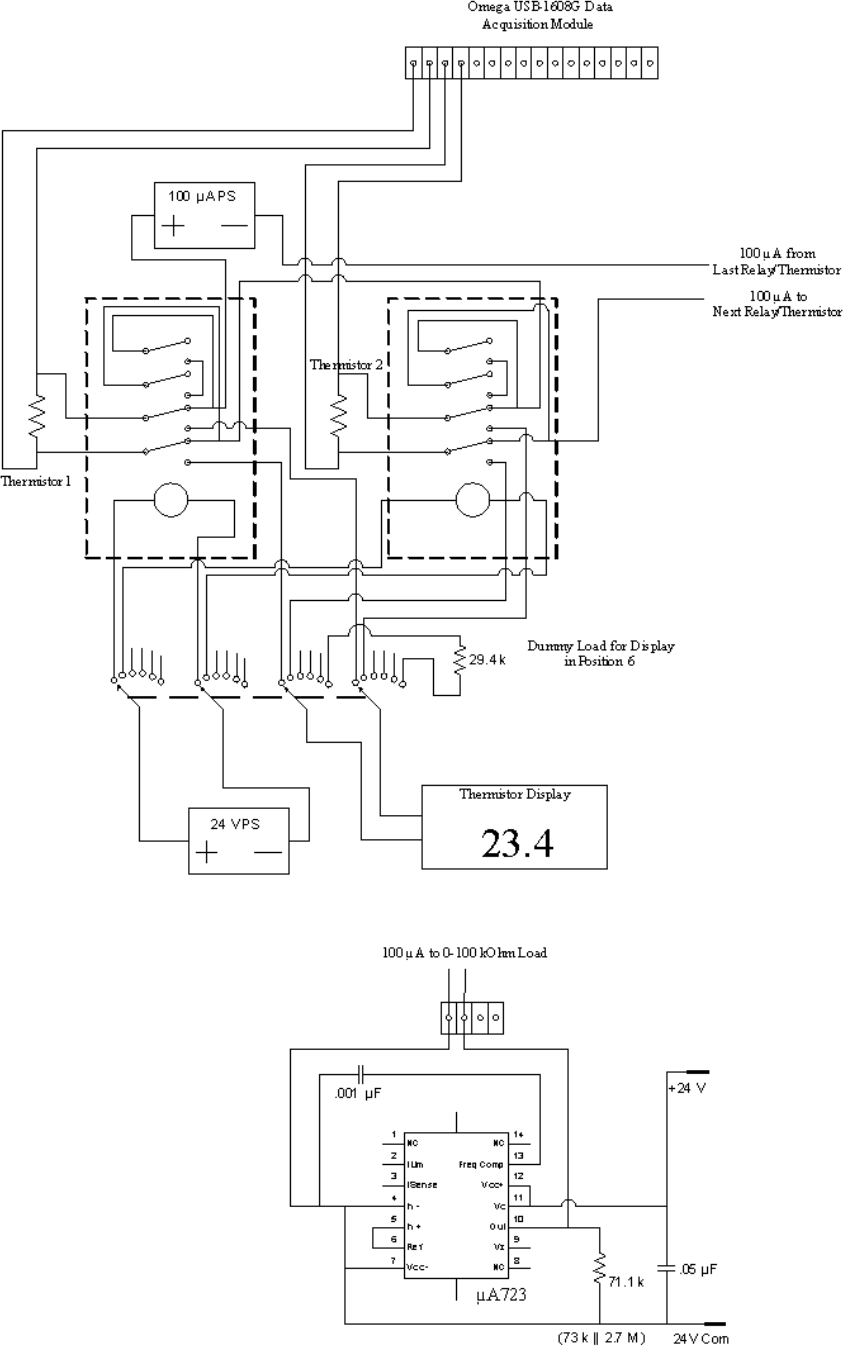
\includegraphics[height=.9\textheight]{./img/subsystem-thermistor-schematic.png}
 % subsystem-thermistor-schematic.png: 0x0 pixel, 2870220dpi, 0.00x0.00 cm, bb=
 \caption{Schematic of thermistor system.}
 \label{fig:subsystem-thermistor-schematic}
\end{figure}
\begin{figure}[!htbp]
 \centering
 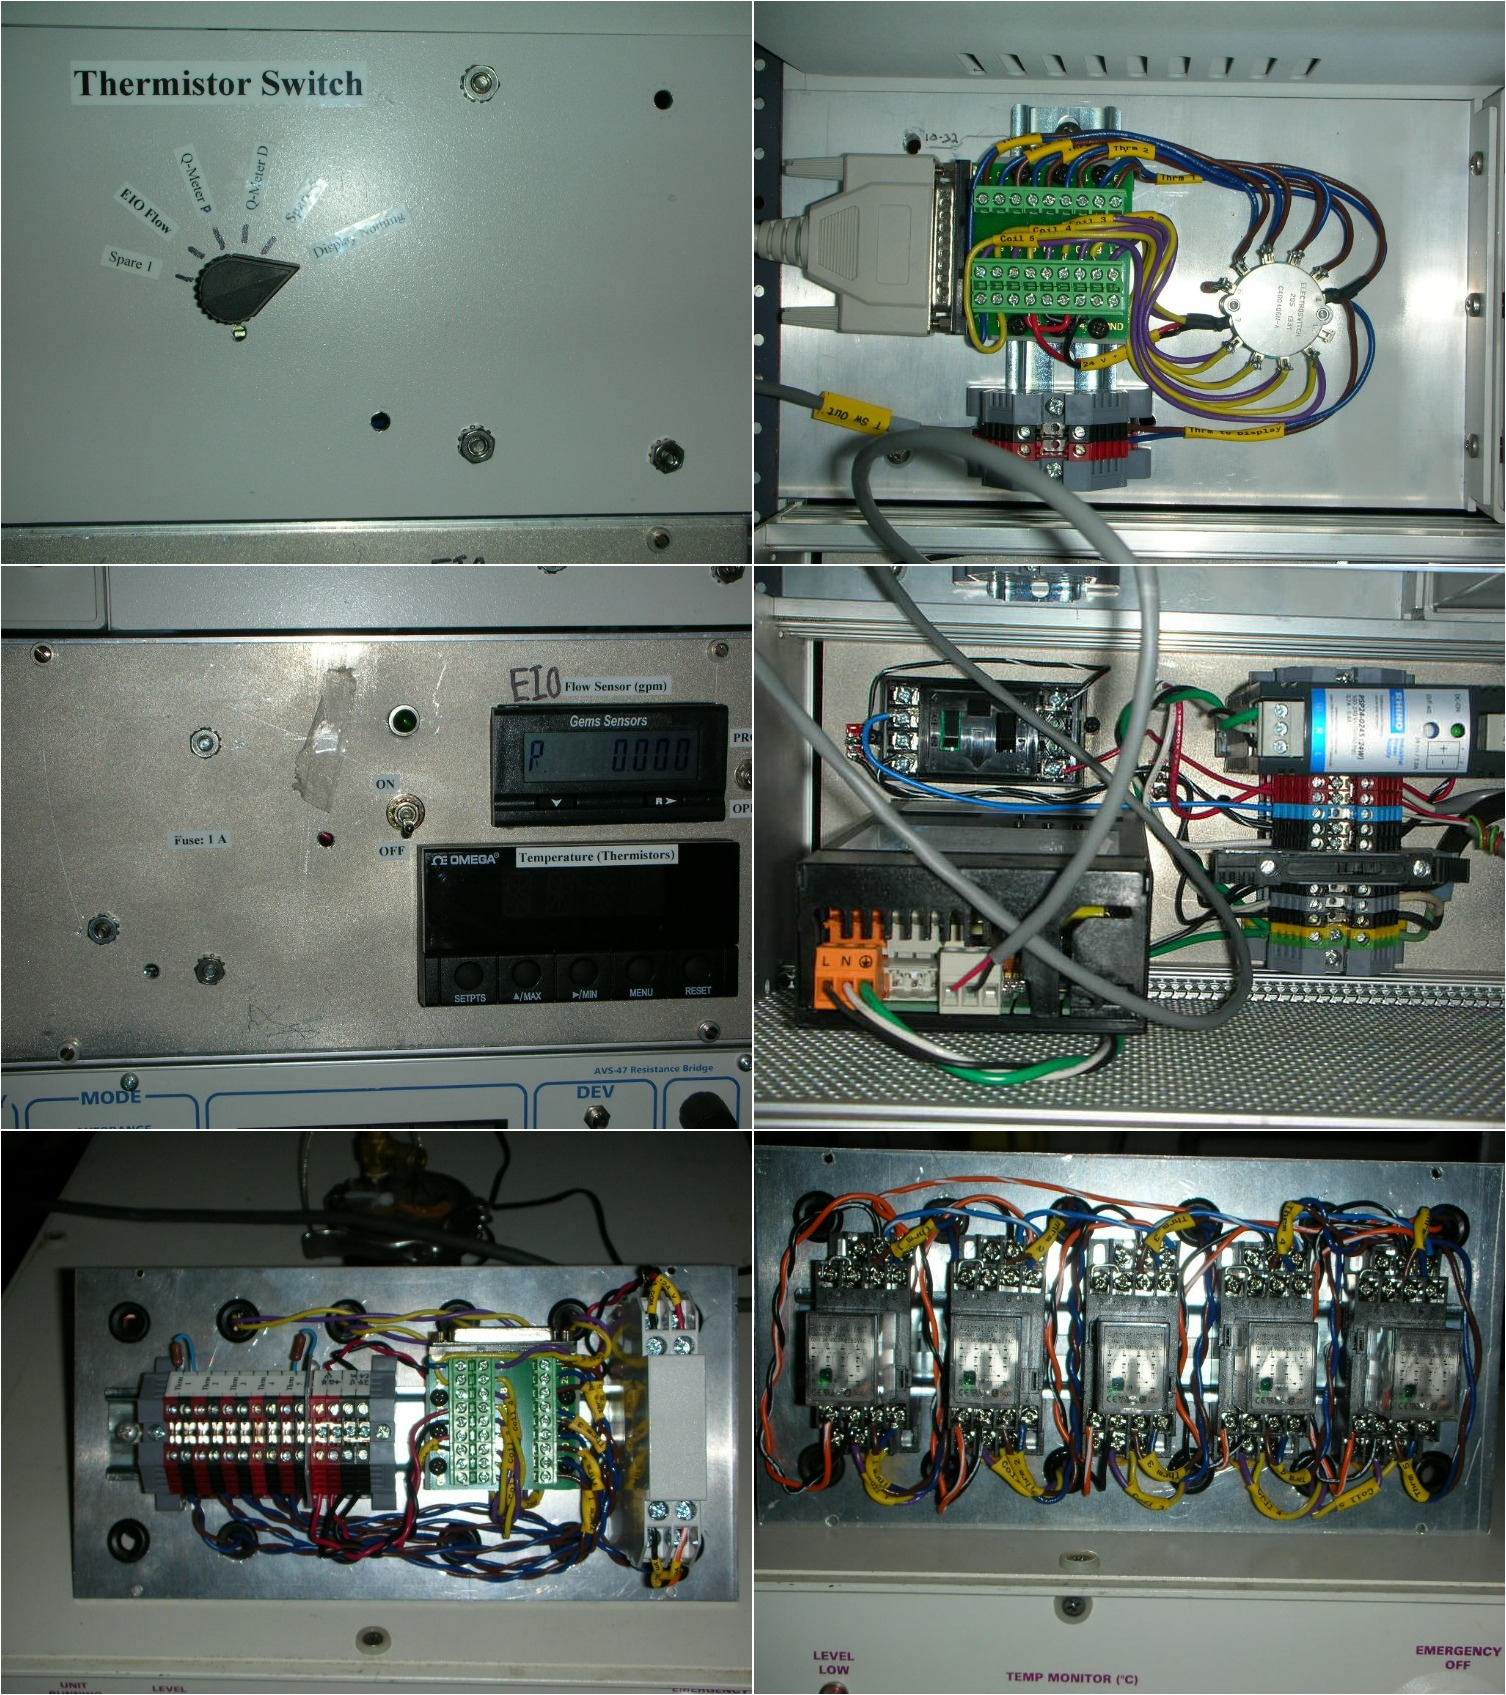
\includegraphics[width=\textwidth]{./img/subsystem-thermistor-photos.png}
 % subsystem-thermistor-photos.png: 0x0 pixel, 0dpi, 0.00x0.00 cm, bb=
 \caption{Photos of thermistor system.}
 \label{fig:subsystem-thermistor-photos}
\end{figure}

\section{IVC Manifold}
TODO: purpose of the IVC manifold, schematic diagram, instructions for turning on vacuum pump

\section{OVC Manifold}
TODO: purpose of the OVC manifold, diagram, photos, HiCube information